\documentclass[11pt]{article}

%% PACKAGES
\usepackage{graphicx}
\usepackage[printonlyused]{acronym}
\usepackage{float}
\usepackage[colorlinks=false]{hyperref}
\usepackage{tabularx}
\usepackage{caption}
\usepackage[margin=1.0in]{geometry}
\usepackage{tocloft}
\usepackage{listings}

\lstset{basicstyle=\small\ttfamily,columns=flexible,breaklines=true,xleftmargin=-0.5in,keepspaces=true}

\setcounter{tocdepth}{3}
\setcounter{secnumdepth}{3}

\makeatletter
\g@addto@macro\normalsize{%
  \setlength\abovedisplayskip{0.25pt}
  \setlength\belowdisplayskip{0.25pt}
  \setlength\abovedisplayshortskip{0.25pt}
  \setlength\belowdisplayshortskip{0.25pt}
}
\makeatother

\setlength{\parskip}{\baselineskip}

%% GRAPHICS PATH
\graphicspath{{../../../shared_latex_inputs/images}{../../../shared_latex_inputs/graphs}}

\newcommand{\acposs}[1]{%
	\expandafter\ifx\csname AC@#1\endcsname\AC@used
	\acs{#1}'s%
	\else
	\aclu{#1}'s (\acs{#1}'s)%
	\fi
}

\title{\Huge EMTG Tutorial: Config Files}
\vspace{0.5cm}
\author
{
	Tim Sullivan \thanks{Aerospace Engineer, The Aerospace Corporation}
}
\vspace{0.5cm}

\newcommand{\listofknownissuesname}{\Large List of Known Issues}
\newlistof{knownissues}{mcf}{\listofknownissuesname}

\newcommand{\knownissue}[3]
{
	\refstepcounter{knownissues}
	\par\noindent\textbf{\hyperref[#2_b]{\theknownissues\quad #1}}\label{#2_h}
	\textbf{\hfill\pageref{#2_b}}
	#3
}

\newcommand{\knownissuelabel}[2]
{
	 \phantomsection
  	\hyperref[#2_h]{#1}\def\@currentlabel{\unexpanded{#1}}\label{#2_b}
}

\begin{document}

\begin{titlepage}
\maketitle
\thispagestyle{empty}
\begin{table}[H]
	\centering
	\begin{tabularx}{\textwidth}{|l|l|X|}
		\hline
		\textbf{Revision Date} & \textbf{Author} & \textbf{Description of Change} \\
		\hline
		\date{December 2, 2022} & Tim Sullivan & Initial revision.\\
		\hline
		\date{June 30, 2023} & Joseph Hauerstein & Conversion to \LaTeX.\\ 
		\hline
		\date{August 4, 2023} & Joseph Hauerstein & Addition of Known Issues section.\\ 
		\hline
	\end{tabularx}
\end{table}
\end{titlepage}

\newpage
\tableofcontents
\thispagestyle{empty}
\newpage

\listofknownissues
\thispagestyle{empty}

\knownissue{EMTG incorrectly names the ElectricPropulsionFromMissionOptions variable}{elec_prop_system_name_issue}

\newpage
\clearpage
\setcounter{page}{1}



\section*{List of Acronyms}
\begin{acronym}
%To define the acronym and include it in the list of acronyms: \acro{acronym}{definition}
%To define the acronym and exclude it from the list of acronyms:  \acro{acronym}{definition}
%
%\ac{acronym} Expand and identify the acronym the first time; use only the acronym thereafter
%\acf{acronym} Use the full name of the acronym.
%\{acronym} Use the acronym, even before the first corresponding \ac command
%\acl{acronym}  Expand the acronym without using the acronym itself.
%
%

\acro{ACS}{attitude control system}
\acro{ACO}{Ant Colony Optimization}
\acro{AD}{Automatic Differentiation}
\acro{ADL}{Architecture Design Laboratory}
\acro{AES}{Advanced Exploration Systems}
\acro{AGA}{aerogravity assist}
\acro{ALARA}{As Low As Reasonably Achievable}
\acro{API}{application programming interface}
\acro{BB}{branch and bound}
\acro{BVP}{Boundary Value Problem}
\acro{CATO}{Computer Algorithm for Trajectory Optimization}
\acro{CL}{confidence level}
\acro{CONOPS}{concept of operations}
\acro{COV}{Calculus of Variations}
\acro{D/AV}{Descent/Ascent Vehicle}
\acro{DE}{Differential Evolution}
\acro{DLA}{Declination of Launch Asymptote}
\acro{RLA}{Right Ascension of Launch Asymptote}
\acro{RA}{right ascension}
\acro{DEC}{declination}
\acro{DPTRAJ/ODP}{Double Precision Trajectory and Orbit Determination Program}
\acro{DSH}{Deep Space Habitat}
\acro{DSN}{Deep Space Network}
\acro{DSMPGA}{Dynamic-Size Multiple Population Genetic Algorithm}
\acro{EB}{Evolutionary Branching}
\acro{ECLSS}{environmental control and life support system}
\acro{ELV}{expendable launch vehicle}
\acro{EMME}{Earth to Mars, Mars to Earth}
\acro{EMMVE}{Earth to Mars, Mars to Venus to Earth}
\acro{EMTG}{Evolutionary Mission Trajectory Generator}
\acro{EVMME}{Earth to Venus to Mars, Mars to Earth}
\acro{EVMMVE}{Earth to Venus to Mars, Mars to Venus to Earth}
\acro{ERRV}{Earth Return Re-entry Vehicle}
\acro{FISO}{Future In-Space Operations}
\acro{FMT}{Fast Mars Transfer}
\acro{GASP}{Gravity Assist Space Pruning}
\acro{GCR}{galactic cosmic radiation}
\acro{GRASP}{Greedy Randomized Adaptive Search Procedure}
\acro{GSFC}{Goddard Space Flight Center}
\acro{GTOC}{Global Trajectory Optimization Competition}
\acro{GTOP}{Global Trajectory Optimization Problem}
\acro{HAT}{Human Architecture Team}
\acro{HGGA}{Hidden Genes Genetic Algorithm}
\acro{IMLEO}{Initial Mass in \acl{LEO}}
\acro{IPOPT}{Interior Point OPTimizer}
\acro{ISS}{International Space Station}
\acro{JHUAPL}{Johns Hopkins University Applied Physics Laboratory}
\acro{JSC}{Johnson Space Center}
\acro{KKT}{Karush-Kuhn-Tucker}
\acro{LEO}{Low Earth Orbit}
\acro{LRTS}{lazy race tree search}
\acro{MONTE}{Mission analysis, Operations, and Navigation Toolkit Environment}
\acro{MCTS}{Monte Carlo tree search}
\acro{MGA}{Multiple Gravity Assist}
\acro{MIRAGE}{Multiple Interferometric Ranging Analysis using GPS Ensemble}
\acro{MOGA}{Multi-Objective Genetic Algorithm}
\acro{MOSES}{Multiple Orbit Satellite Encounter Software}
\acro{MPI}{message passing interface}
\acro{MPLM}{Multi-Purpose Logistics Module}
\acro{MSFC}{Marshall Space Flight Center}
\acro{NELLS}{NASA Exhaustive Lambert Lattice Search}
\acro{NSGA}{Non-Dominated Sorting Genetic Algorithm}
\acro{NSGA-II}{Non-Dominated Sorting Genetic Algorithm II}
\acro{NHATS}{Near-Earth Object Human Space Flight Accessible Targets Study}
\acro{NTP}{Nuclear Thermal Propulsion}
\acro{OD}{orbit determination}
\acro{OOS}{On-Orbit Staging}
\acro{PCC}{Pork Chop Contour}
\acro{PEL}{permissible exposure limits}
\acro{PLATO}{PLAnetary Trajectory Optimization}
\acro{REID}{risk of exposure-induced death}
\acro{RTBP}{Restricted Three Body Problem}
\acro{SA}{Simulated Annealing}
\acro{SLS}{Space Launch System}
\acro{SNOPT}{Sparse Nonlinear OPTimizer}
\acro{SOI}{sphere of influence}
\acro{SPE}{solar particle events}
\acro{SQP}{sequential quadratic programming}
\acro{SRAG}{Space Radiation Analysis Group}
\acro{TEI}{Trans-Earth Injection}
\acro{TOF}{time of flight}
\acro{TPBVP}{Two Point Boundary Value Problem}
\acro{TMI}{Trans-Mars Injection}
\acro{VARITOP}{Variational calculus Trajectory Optimization Program}
\acro{VILM}{v-infinity leveraging maneuver}
\acro{MOI}{Mar Orbit Injection}
\acro{PCM}{Pressurized Cargo Module}
\acro{STS}{Space Transportation System}
\acro{EDS}{Earth Departure Stage}
\acro{NEO}{near-Earth asteroid}
\acro{IDC}{Integrated Design Center}
\acro{SEP}{solar-electric propulsion}
\acro{SRP}{solar radiation pressure}
\acro{NEP}{nuclear-electric propulsion}
\acro{REP}{radioisotope-electric propulsion}
\acro{DRM}{Design Reference Missions}

\acro{EDL}{entry, descent, and landing}
\acro{ASCII}{American Standard Code for Information Interchange}
\acro{AU}{Astronomical Unit}
\acro{BWG}{Beam Waveguides}
\acro{CCB}{Configuration Control Board}
\acro{CMO}{Configuration Management Office}
\acro{CODATA}{Committee on Data for Science and Technology}
\acro{DEEVE}{Dynamically Equivalent Equal Volume Ellipsoid}
\acro{DRA}{Design Reference Asteroid}
\acro{EME2000}{Earth Centered, Earth Mean Equator and Equinox of J2000 (Coordinate Frame)}
\acro{EOP}{Earth Orientation Parameters}
\acro{ET}{Ephemeris Time}
\acro{FDS}{Flight Dynamics System}
\acro{FTP}{File Transfer Protocol}
\acro{GSFC}{Goddard Space Flight Center}
\acro{PI}{Principal Investigator}
\acro{HEF}{High Efficiency}
\acro{IAG}{International Association of Geodesy}
\acro{IAU}{International Astronomical Union}
\acro{IERS}{International Earth Rotation and Reference Systems Service}
\acro{ICRF}{International Celestial Reference Frame}
\acro{ITRF}{International Terrestrial Reference System}
\acro{IOM}{Interoffice Memorandum}
\acro{JD}{Julian Date}
\acro{JPL}{Jet Propulsion Laboratory}
\acro{LM}{Lockheed Martin}
%\acro{LP150Q}{}
%\acros{LP100K}{}
\acro{MAVEN}{Mars Atmosphere and Volatile EvolutioN}
\acro{MJD}{Modified Julian Date}
\acro{MOID}{Minimum Orbit Intersection Distance}
\acro{MPC}{Minor Planet Center}
\acro{NASA}{National Aeronautics and Space Administration}
\acro{NDOSL}{\ac{NASA} Directory of Station Locations}
\acro{NEA}{near-Earth asteroid}
\acro{NEO}{near-Earth object}
\acro{NIO}{Nav IO}
\acro{OSIRIS-REx}{Origins Spectral Interpretation Resource Identification Security-Regolith Explorer}
\acro{PHA}{Potentially Hazardous Asteroid}
\acro{PHO}{Potentially Hazardous Object}
\acro{SBDB}{Small-Body Database}
\acro{SI}{International System of Units}
\acro{SPICE}{Spacecraft Planet Instrument Camera-matrix Events}
\acro{SPK}{SPICE Kernel}
\acro{SRC}{Sample Return Capsule}
\acro{SSD}{Solar System Dynamics}
\acro{STK}{Systems Tool Kit}
\acro{TAI}{International Atomic Time}
\acro{TBD}{To Be Determined}
\acro{TBR}{To Be Reviewed}
\acro{TCB}{Barycentric Coordinate Time}
\acro{TDB}{Temps Dynamiques Barycentrique, Barycentric Dynamical Time}
\acro{TDT}{Terrestrial Dynamical Time}
\acro{TT}{Terrestrial Time}
\acro{URL}{Uniform Resource Locator}
\acro{UT}{Universal Time}
\acro{UT1}{Universal Time Corrected for Polar Motion}
\acro{UTC}{Coordinated Universal Time}
\acro{USNO}{U. S. Naval Observatory}
\acro{YORP}{Yarkovsky-O'Keefe-Radzievskii-Paddack}

\acro{NLP}{nonlinear program}
\acro{MBH}{monotonic basin hopping}
\acro{MBH-C}{monotonic basin hopping with Cauchy hops}
\acro{FBS}{forward-backward shooting}
\acro{MGALT}{Multiple Gravity Assist with Low-Thrust}
\acro{MGALTS}{Multiple Gravity Assist with Low-Thrust using the Sundman transformation}
\acro{MGA-1DSM}{Multiple Gravity Assist with One Deep Space Maneuver}
\acro{MGAnDSMs}{Multiple Gravity Assist with \textit{n} Deep-Space Maneuvers using Shooting}
\acro{PSFB}{Parallel Shooting with Finite-Burn}
\acro{PSBI}{Parallel Shooting with Bounded Impulses}
\acro{FBLT}{Finite-Burn Low-Thrust}
\acro{FBLTS}{Finite-Burn Low-Thrust using the Sundman transformation}
\acro{ESA}{European Space Agency}
\acro{ACT}{Advanced Concepts Team}
\acro{IRAD}{independent research and development}
\acro{Isp}[$\text{I}_{sp}$]{specific impulse}
\acro{C3}[$C_3$]{hyperbolic excess energy}
\acro{GA}{genetic algorithm}
\acro{GALLOP}{ Gravity Assisted Low-thrust Local Optimization Program}
\acro{MALTO}{Mission Analysis Low-Thrust Optimization}
\acro{PaGMO}{Parallel Global Multiobjective Optimizer}
\acro{FRA}{feasible region analysis}
\acro{CP}{conditional penalty}
\acro{HOC}{hybrid optimal control}
\acro{HOCP}{hybrid optimal control problem}
\acro{PSO}{particle swarm optimization}
\acro{SEPTOP}{Solar Electric Propulsion Trajectory Optimization Program}
\acro{STOUR}{Satellite Tour Design Program}
\acro{STOUR-LTGA}{Satellite Tour Design Program - Low Thrust, Gravity Assist}
\acro{PaGMO}{Parallel Global Multiobjective Optimizer}
\acro{SDC}{static/dynamic control}
\acro{DDP}{Differential Dynamic Programming}
\acro{HDDP}{Hybrid Differential Dynamic Programming}
\acro{ACT}{Advanced Concepts Team}
\acro{GMAT}{General Mission Analysis Toolkit}
\acro{BOL}{beginning of life}
\acro{EOL}{end of life}
\acro{KSC}{Kennedy Space Center}
\acro{VSI}{variable \ac{Isp}}
\acro{RTG}{radioisotope thermal generator}
\acro{ASRG}{advanced Stirling radiosotope generator}
\acro{ARRM}{Asteroid Robotic Redirect Mission}
\acro{AATS}{Alternative Architecture Trade Study}
\acro{PPU}{power processing unit}
\acro{STM}{state transition matrix}
\acro{MTM}{maneuver transition matrix}
\acro{HPTM}{half-phase transition matrix}
\acro{BCI}{body-centered inertial}
\acro{BCF}{body-centered fixed}
\acro{UTTR}{Utah Test and Training Range}
\acro{EPV}{equatorial projection of $\mathbf{v}_\infty$}
\acro{KBO}{Kuiper belt object}
\acro{DSM}{deep-space maneuver}
\acro{BPT}{body-probe-thrust}
\acro{4PL}{four parameter logistic}
\acro{BCF}{body-centered fixed}
\acro{COE}{classical orbit elements}
\acro{GSL}{Gnu Scientific Library}
\acro{NEXT}{NASA's Evolutionary Xenon Thruster}

\acro{SMA}{semi-major axis}
\acro{ECC}{eccentricity}

\acro{GSAD}{Ghosh Sparse Algorithmic Differentiation}

\end{acronym}

% --------------------------------------------------------------------------------------------------------------------------
% --------------------------------------------------------------------------------------------------------------------------


%%%%%%%%%%%%%%%%%%%%%
\section{Introduction}
\label{sec:introduction}
%%%%%%%%%%%%%%%%%%%%%

\ac{EMTG} can model performance characteristics of spacecraft and launch vehicles using text files separate from the main \ac{EMTG} options file. These text files can be configuration controlled and shared across missions. So far, you’ve only briefly mentioned the configuration of the launch vehicle and spacecraft. This tutorial will dive deeper into the methods for modeling vehicle performance in \ac{EMTG} though explaining the different options in these configuration files.

\noindent There are three basic ways to set up spacecraft hardware in \ac{EMTG}, which can be seen on the ``Spacecraft Options'' tab of the PyEMTG \acs{GUI} under the ``Spacecraft model type'' label: ``0:  Assemble from libraries'', ``1: Read .emtg\_spacecraftoptions file'', and ``2: Assemble from missionoptions object''. In the (Low/O)SIRIS-REx tutorials you used the ``2: Assemble from missionoptions object'' method by setting spacecraft values in PyEMTG. Method ``1: Read .emtg\_spacecraftoptions file'' uses a single file to set all spacecraft mass, power, and propulsion options. Method ``0: Assemble from libraries'' uses separate propulsion and power system library files. The system to use is then selected in the ``Spacecraft Options'' tab. This tutorial will focus on using Method 1, the Spacecraft Options file. 

\noindent Launch vehicles must be configured using the Launch Vehicle Options file.

\noindent More information can be found in the \ac{GMAT} Optimal Control Specification, Chapter 6: \ac{EMTG} Spacecraft File Specification and Section 4.8.5: Format of \ac{EMTG} Spacecraft File, Chapter 5 of the \ac{EMTG} Software Design Document, and the example configuration files provided with this tutorial.

%%%%%%%%%%%%%%%%%%%%%
\section{Spacecraft Options}
\label{sec:spacecraft_options}
%%%%%%%%%%%%%%%%%%%%%

In the LowSIRIS-REx tutorial, you specified the thrust and power systems of the spacecraft directly in PyEMTG. This section will go over how to do this using the spacecraft options file. 
 
\noindent The spacecraft options file layout consists of sections of data called ``blocks''. The first block contains some global data and is identified by the line \texttt{\#BeginSpacecraftBlock}. The spacecraft block is followed by one or more stage blocks, each of which is identified by the line \texttt{\#BeginStageBlock}. (In \ac{EMTG}, ``staging'' means to change the spacecraft hardware characteristics. Staging events are controlled by check boxes in the upper right of the ``Journey Options'' tab in PyEMTG. Creating a staging event moves \ac{EMTG} from the current stage block to the next stage block.) Each stage block is independent of data in other stage blocks and contains some unblocked data, power library data identified by the line \texttt{\#BeginStagePowerLibraryBlock}, and propulsion library data identified by the line \texttt{\#BeginStagePropulsionLibraryBlock}. Thus, a two-stage spacecraft options file would be setup as follows:

\begin{itemize}
	\item Spacecraft block data
	\item Stage 1 block
	\begin{itemize}
		\item Unblocked data for stage 1
		\item Power library blcok data for stage 1
		\item Propulsion library block data for stage 1
	\end{itemize}
	\item Stage 2 block
	\begin{itemize}
		\item Unblocked data for stage 2
		\item Power library block data for stage 2
		\item Propulsion library block data for stage 2
	\end{itemize}
\end{itemize}

%%%%%%%%%%%%%%%%%%%%%
\subsection{Spacecraft Block}
\label{sec:spacecraft_block}
%%%%%%%%%%%%%%%%%%%%%

The spacecraft block data section sets the name of the spacecraft and enables or disables maximum values on the spacecraft electrical and chemical tanks, as well as the spacecraft dry mass. The spacecraft block also provides the required minimum/maximum values for constraints that are enabled. The lines and expected data types are shown in Table \ref{tab:spacecraft_block_data}.

\begin{table}[H]
	\begin{small}
		\begin{tabularx}{\linewidth} { >{\arraybackslash}p{4em} >{\arraybackslash} X >{\arraybackslash} X}
			\hline
			Line number & Line name & Data type \\
			\hline 
			1 & Name & String \\ 
			2 & EnableGlobalElectricPropellant-TankConstraint & Boolean integer \\ 
			3 & EnableGlobalChemicalPropella-ntTankConstraint & Boolean integer \\
			4 & EnableGlobalDryMassConstrai-nt & Boolean integer \\
			5 & GlobalElectricPropellantTankC-apacity & Real (kg) \\ 
			6 & GlobalFuelTankCapacity & Real (kg)\newline \\ 
			7 & GlobalOxidizerTankCapacity & Real (kg)\newline \\
			8 & GlobalDryMassLowerBound & Real (\( \mathrm{kg \geq 0 \leq GlobalDryMassBounds[1] } \)) \\
			9 & GlobalDryMassUpperBound & Real (\( \mathrm{kg \geq GlovalDryMassBounds[0]} \)) \\ 
 			\hline
		\end{tabularx}
	\end{small}
	\caption{\label{tab:spacecraft_block_data}Spacecraft Block Data.}
\end{table}

\noindent The bounds values are only considered if the corresponding constraint is active. For example, the spacecraft block in Figure \ref{fig:example_spacecraft_block_section} would only constrain the electric propellant tank since the constraint is set to ``1''. Even though the chemical fuel tank capacity has a value of 100 kg, that constraint would not be active because the corresponding option to enable the chemical tank constraint is set to ``0''.

\begin{figure}
	\centering
	\fbox{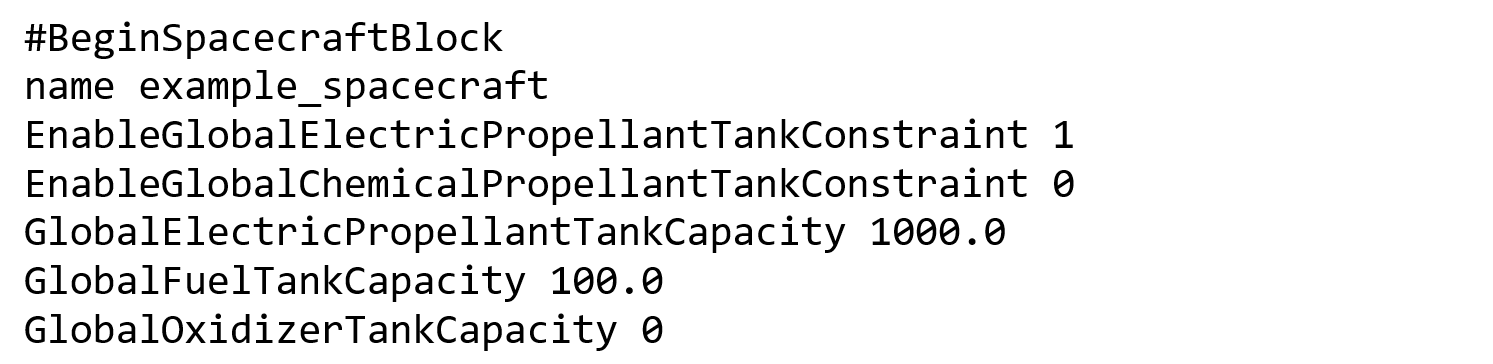
\includegraphics[width=0.7\linewidth]{Config_Files_example_spacecraft_block_section.png}}
	\caption{\label{fig:example_spacecraft_block_section}Example Spacecraft Block Section.}
\end{figure}

%%%%%%%%%%%%%%%%%%%%%
\subsection{Stage Unblocked Data}
\label{sec:stage_unblocked_data}
%%%%%%%%%%%%%%%%%%%%%

After the Spacecraft Block section, there are one or more ``Stage Block'' sections. Each Stage Block begins with ``Unblocked'' information. This section is similar to the Spacecraft Block section, specifying stage masses, constraints, and maximum masses for the fuel tanks. There are also lines for number of thrusters and throttle sharpness. The line items and expected data types are shown in Table \ref{tab:stage_unblocked_data}.

\begin{table}
	\begin{small}
		\begin{tabularx}{\linewidth} { >{\arraybackslash}p{4em} >{\arraybackslash} X >{\arraybackslash}p{10em}}
			\hline
			Line number & Line name & Data type \\
			\hline 
			1 & Name & String \\ 
			2 & BaseDryMass & Real (kg) \\ 
			3 & AdapterMass &  Real (kg) \\
			4 & EnableElectricPropellantTankConstraint & Boolean integer \\
			5 & EnableChemicalPropellantTankConstraint & Boolean integer \\ 
			6 & EnableDryMassConstraint & Boolean integer \\ 
			7 & ElectricPropellantTankCapacity & Real (kg) \\
			8 & ChemicalFuelTankCapacity & Real (kg) \\
			9 & ChemicalOxidizerTankCapacity & Real (kg) \\
			10 & ThrottleLogic & Integer(1: min number of thrusters, 2: max number of thrusters \\
			11 & ThrottleSharpness & Real (kg) \\
			12 & PowerSystem & String (name of power system) \\
			13 & ElectricPropulsionSystem & String (name of propulsion system) \\
			14 & ChemicalPropulsionSystem & String (name of propulsion system) \\ 
 			\hline
		\end{tabularx}
	\end{small}
	\caption{\label{tab:stage_unblocked_data}Stage Unblocked Data.}
\end{table}

\noindent The Stage Block section has a dry mass constraint Boolean option but no entry for the bounds like in the Spacecraft Block section. If \texttt{EnableDryMassConstraint == 1}, a constraint is created specifying that the final mass at the end of the stage must be greater than the required mass at the end of the stage. The required mass is the sum of the stage BaseDryMass, stage electric propulsion system mass, stage chemical propulsion system mass, stage power system mass, electric propellent mass margin, chemical fuel mass margin, chemical oxidizer mass margin. The fractional margins are set in PyEMTG in the ``Spacecraft Options'' tab under the ``Margins'' header.

\noindent Throttle sharpness is how quickly the thruster transitions between different settings. A larger value indicates a steeper curve and faster transition. The throttle sharpness model uses an approximation of the Heaviside step function where k is the throttle sharpness and x is a power parameter. A k value of 100 is usually a good rule of thumb. Examples of throttle sharpness curves are shown in Figure \ref{fig:throttle_sharpness}. See Section 5.6.2.4 of the \ac{EMTG} Software Design Document for a more detailed explanation of how throttle sharpness is implemented and used in \ac{EMTG}.

\[H=\frac{1}{1-e^{-2kx}}\]

\begin{figure}[H]
	\centering
	\fbox{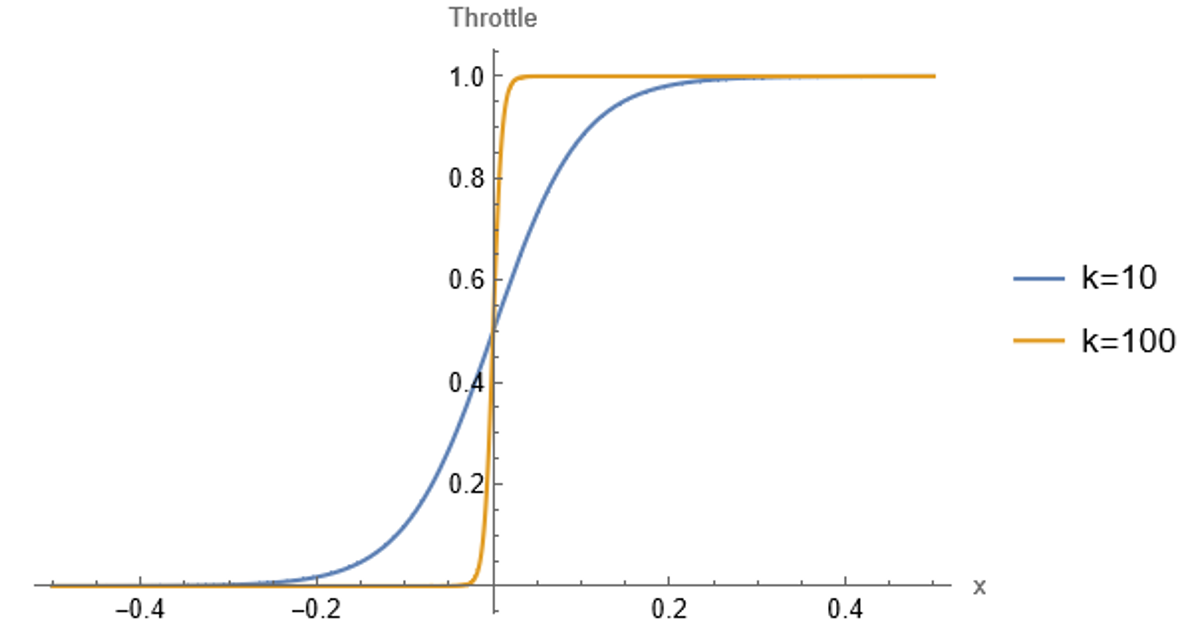
\includegraphics[width=\linewidth]{Config_Files_throttle_sharpness.png}}
	\caption{\label{fig:throttle_sharpness}Throttle Sharpness.}
\end{figure}

\noindent The last lines of the unblocked stage section specify the names of the power, electrical, and chemical propulsion systems being used for this stage. These must correspond to names available in the power and propulsion library blocks for this stage. The library of available power and propulsion systems for the stage are detailed in the next blocks. An example of all stage unblocked data options is shown in Figure \ref{fig:example_stage_unblocked_data}.

\begin{figure}[H]
	\centering
	\fbox{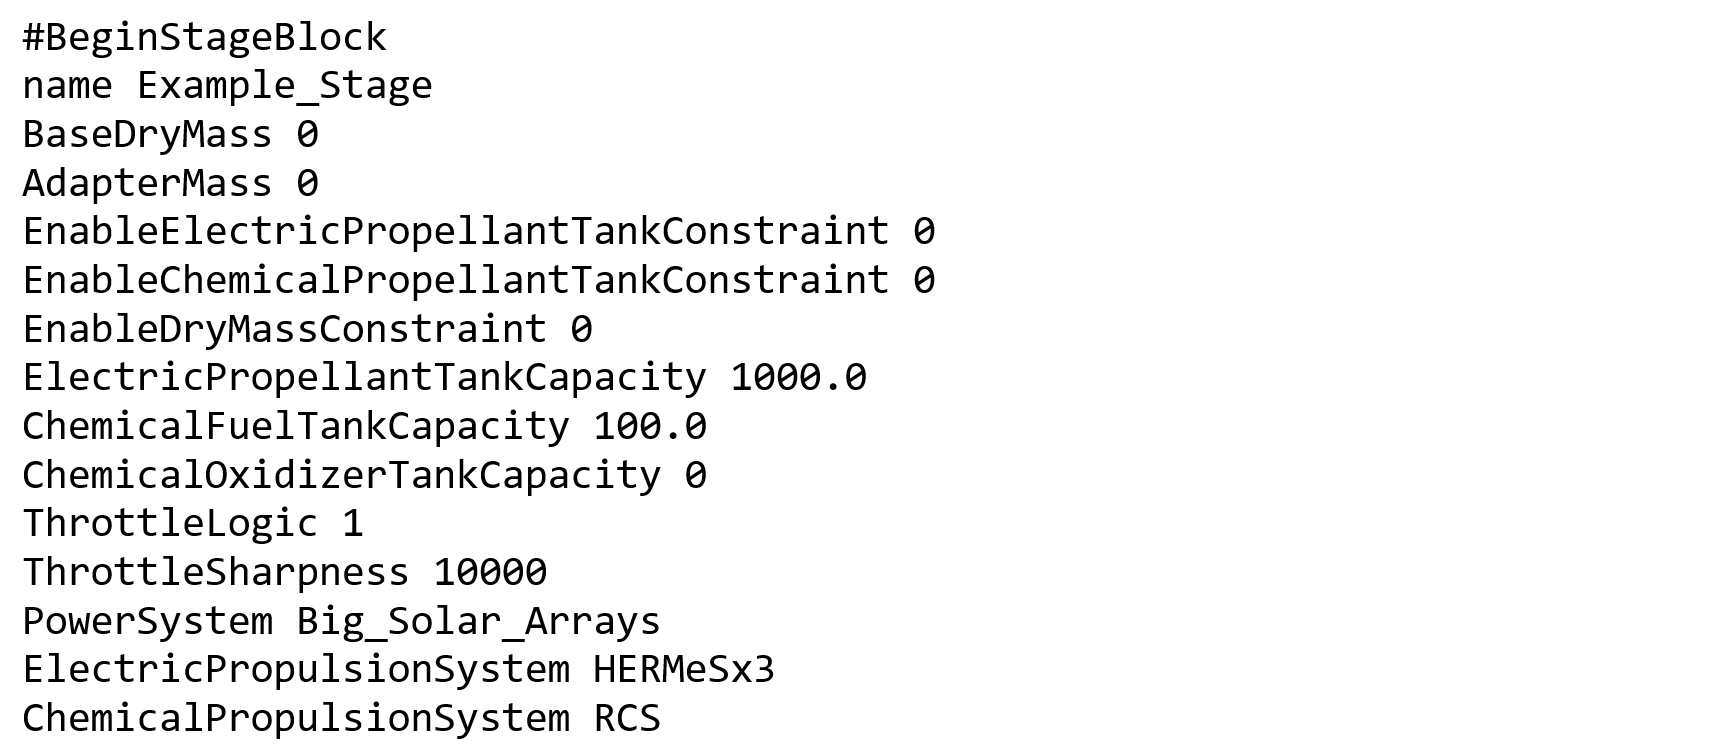
\includegraphics[width=\linewidth]{Config_Files_example_stage_unblocked_data.png}}
	\caption{\label{fig:example_stage_unblocked_data}Example Stage Unblocked Data.}
\end{figure}

%%%%%%%%%%%%%%%%%%%%%
\subsection{Power Library Block}
\label{sec:power_library_block}
%%%%%%%%%%%%%%%%%%%%%

The Power Library Block specifies in text form the set of power options. This is the information that would be set in the PyEMTG ``Power options'' section if ``Spacecraft model type'' were set to ``2: Assemble from missionoptions object'' as in Figure \ref{fig:power_options}. 

\begin{figure}[H]
	\centering
	\fbox{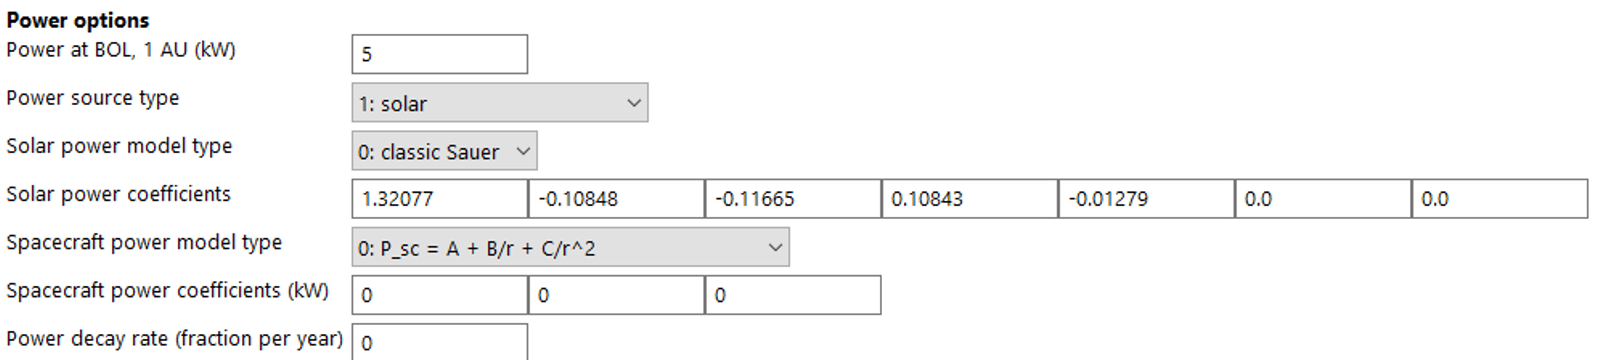
\includegraphics[width=\linewidth]{Config_Files_power_options.png}}
	\caption{\label{fig:power_options}PyEMTG Power Options.}
\end{figure}

\noindent Power systems are specified by a name followed by a series of comma or space-delimited numbers all on one line. A stage can have multiple power systems specified in the Power Library Block by having multiple lines of data, but only the one specified in the Unblocked Stage data as the \texttt{PowerSystem} will be used for that stage. Table \ref{tab:power_system_vars} specifies the parameters and data types for each Power System.

\begin{table}[H]
	\begin{small}
		\begin{tabularx}{\linewidth} { >{\arraybackslash}p{4em} >{\arraybackslash} X >{\arraybackslash}p{10em}}
			\hline
			Index & Variable name & Data type \\
			\hline 
			1 & Name & String \\ 
			2 & SpacecraftPowerSupplyType & Integer (0: Constant, 1: Solar) \\ 
			3 & SpacecraftPowerSupplyCurveType &  (0: Sauer, 1: Polynomial) \\
			4 & SpacecraftBusPowerType & Integer (0: TypeA\_Q-uadratic, \newline 1: TypeB\_Conditional) \\
			5 & P0 & Real (kW) \\
			6 & MassPerkW & Real (kg) \\ 
			7 & DecayRate & Real (1/years) \\
			8-14 & Gamma[0:6] & Real \\
			15-17 & BusPower[0:2] & Real \\
 			\hline
		\end{tabularx}
	\end{small}
	\caption{\label{tab:power_system_vars}Power System Variables.}
\end{table}

%%%%%%%%%%%%%%%%%%%%%
\subsubsection{Power Supply Type and Curve}
\label{sec:power_supply_type_and_curve}
%%%%%%%%%%%%%%%%%%%%%

Items 2, 3, and 5-14 specify the power produced for the propulsion system, while items 4 and 15-17 specify the spacecraft power use for purposes other than electric propulsion. (I.e., a non-zero bus power means that there is some amount of power produced by the spacecraft that cannot be used by the electric propulsion system.) Several options require coefficients of \(r_s\), which is the spacecraft distance from the Sun, measured in \acs{AU}. Additional information, including more detailed equations of how various power quantities are calculated, is available is Section 5.5 of the \ac{EMTG} Software Design Document.

\noindent \textbf{Spacecraft\_Power\_Supply\_Type:} This option is an integer specifying either a constant power supply (0) or one dependent on solar power produced by the spacecraft (1).

\noindent \textbf{Spacecraft\_Power\_Supply\_Curve\_Type:} If the power supply type is set to solar, this option specifies the type of solar power curve, either Sauer or polynomial. The coefficients, \(\gamma_i\), for both types are specified in indices 8-14 for polynomial curve or 8-11 for Sauer. \(P_{Generated}\) is in kW.

0: Sauer \[ P_{Generated}=\frac{P_0}{r_s^2}\left(\frac{\gamma_0+\frac{\gamma_1}{r_s}+\frac{\gamma_2}{r_s^2}}{1+\gamma_3r_s+\gamma_4r_s^2}\right) \]

1: Polynomial \[ P_{Generated}=P_0\cdot\sum_{i=0}^6\gamma_ir_s^{i-2} \]

\noindent \textbf{P0:} This is the power in kW delivered at 1 \acs{AU} at the start of the mission.

\noindent \textbf{mass\_per\_kW:} This is the spacecraft stage mass increase per kW power delivered.

\noindent \textbf{decay\_rate:} Decay rate of the power supplied by the power supply curve or constant power source. The units are 1/years and the change in supplied power is given by the following equation where \(t\) is in years,

\[ P_{Generated} = P_{Generated,nominal}e^{-\mathrm{decay\_rate}\cdot (t-t_{ref})} \]

\noindent The epoch \(t_{ref}\) is set in PyEMTG on the ``Spacecraft Options'' tab in the ``Power Source Decay Reference Epoch'' text box.

\noindent \textbf{gamma[0:6]:} Coefficients for the power supply curves, as described above.

%%%%%%%%%%%%%%%%%%%%%
\subsubsection{Bus Power}
\label{sec:bus_power}
%%%%%%%%%%%%%%%%%%%%%

The bus power options specify the power used by the spacecraft, which is \textit{not} available to be used by the electric propulsion system.

\noindent \textbf{Spacecraft\_Bus\_Power\_Type:} Like power supply type, there are two different options for modeling the spacecraft bus power type. The coefficients for each are specified by the values in indices 15-17.

0: quadratic \[ P_{Bus} = \sum_{i=0}^2 \mathrm{bus\_power}_i / r_s^i \]

1: conditional 

\[ \left\{ \begin{array}{l} P_{Bus} = \mathrm{bus\_power[0]},  P_{Provided} > \mathrm{bus\_power[0]} \\ P_{Bus} = \mathrm{bus\_power[0]} + \mathrm{bus\_power[1]} \cdot \left(\mathrm{bus\_power[2]} - P_{Provided}\right), \mathrm{otherwise} \end{array} \right. \]

\noindent \textbf{BusPower[0:2]:} The coefficients for either bus power type equation. 

\noindent In practice, early designs frequently make use of simple power models (i.e., lots of zeros in the power system specification line). However, as the overall design increases in fidelity, moving to a more accurately modeled power system helps maintain realism in the trajectory design. An example of a simple power model is shown in Figure \ref{fig:simple_power_model}.

\begin{figure}[H]
	\centering
	\fbox{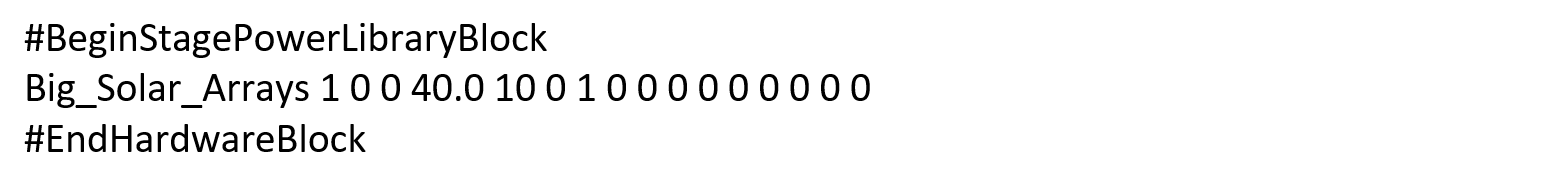
\includegraphics[width=\linewidth]{Config_Files_simple_power_model.png}}
	\caption{\label{fig:simple_power_model}Power Library Block Example for a Simple Power Model.}
\end{figure}

%%%%%%%%%%%%%%%%%%%%%
\subsection{Propulsion Library Block}
\label{sec:propulsion_library_block}
%%%%%%%%%%%%%%%%%%%%%

The Propulsion Library Block specifies in text form the set of propulsion system options. These are the options that would be set in the ``Propulsion options'' section of the PyEMTG \acs{GUI} when ``Spacecraft model type'' is set to ``2: Assemble from missionoptions object'' as shown in Figure \ref{fig:prop_options_continuous_isp}. There many more types of thrusters than there are power systems, and it’s worth selecting different types using the ``Engine type'' option in PyEMTG to see the options which are valid for each thruster type. Additional information is available is Section 5.6 of the \ac{EMTG} Software Design Document.

\begin{figure}
	\centering
	\fbox{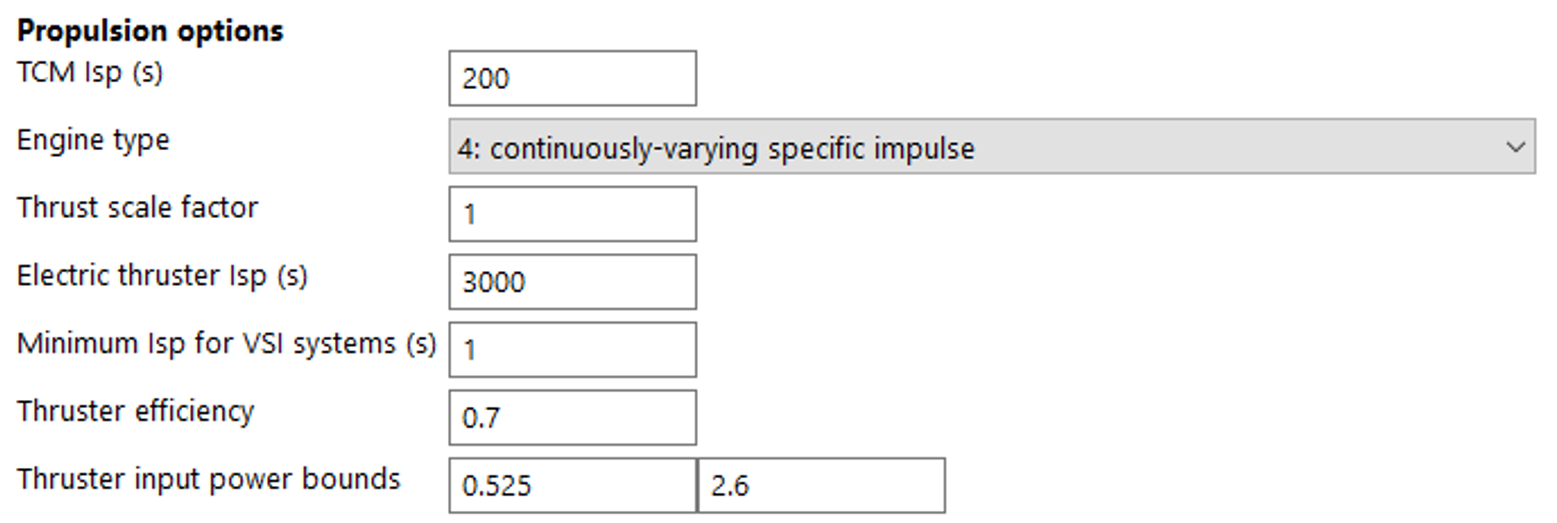
\includegraphics[width=\linewidth]{Config_Files_propulsions_options_for_continuously_varying_isp.png}}
	\caption{\label{fig:prop_options_continuous_isp}PyEMTG Propulsion Options for Continuously-varying Isp.}
\end{figure}

\noindent Like the Power Library Block, the Propulsion Library Block contains one or more rows with the name of the propulsion system and a series of parameters that specify its performance. These are specified in Table \ref{tab:prop_system_vars}.

\begin{table}[H]
	\begin{small}
		\begin{tabularx}{\linewidth} { >{\arraybackslash}p{4em} >{\arraybackslash}p{13em} >{\arraybackslash} X }
			\hline
			Index & Variable name & Data type \\
			\hline 
			1 & Name & String \\ 
			2 & ThrusterMode & Integer (0: ConstantThrustIsp, 1: FixedEfficiencyCSI, 2: FixedEfficiencyVSI, 3: Poly1D, 4: SteppedHThrust1D, 5: SteppedLMdot1D, 6: SteppedHIsp1D, 7: SteppedHefficiency1D, 8: SteppedFullSet1D,, 9: Stepped2D, 10: Poly2D) \\ 
			3 & ThrottleTableFile &  String (``none'' or path to external file) \\
			4 & MassPerString & Real (kg) \\
			5 & NumberOfStrings & Integer \\
			6 & Pmin & Real (kW) \\ 
			7 & Pmax & Real (kW) \\
			8 & ConstantThrust & Real (N) \\
			9 & ConstantIsp & Real (s) \\
			10 & MinimumIsp/MonopropIsp & Real (s) \\ 
			11 & FixedEfficiency & Real [0,1] \\ 
			12 & MixtureRatio & Real [0,1] \\ 
			13 & ThrustScaleFactor & Real (\(\mathrm{\geq 0}\) \\ 
			14-20 & ThrustCoefficients[0:6] & Real (mN) \\ 
			21-27 & MassFlowCoefficients[0:6] & Real (mg/s) \\ 
 			\hline
		\end{tabularx}
	\end{small}
	\caption{\label{tab:prop_system_vars}Propulsion System Variables.}
\end{table}

\noindent \textbf{ThrusterMode:} Integer specifying type of thruster. Not all variables are relevant for each type of thruster.

\noindent \textbf{ThrottleTableFile:} \ac{EMTG} can read in a file specifying thruster throttle levels and parameters at each level. This capability is beyond the scope of this tutorial. More information is available in the \ac{GMAT} Optimal Control Specification section 4.8.6 and Section 5.6 of the \ac{EMTG} Software Design Document.

\noindent \textbf{MassPerString:} The mass of the propulsion system for one thruster ``string''. The total mass of the propulsion system for a given stage is MassPerString * NumberOfStrings. 

\noindent \textbf{NumberOfStrings:} The number of propulsion system ``strings''. In other words, the number of thrusters. The logic for the number of strings/thrusters to use is set using PyEMTG in the ``Spacecraft Options'' tab using the ``Throttle logic mode'' setting. The number of strings/thrusters that can be used depends on the amount of power available. For example, two strings/thrusters cannot be operated if there is only enough power for one string/thruster. \ac{EMTG} uses Heaviside step function approximations to continuously transition in an almost-discrete way from n strings to n+1 or n-1 strings.

\noindent \textbf{Pmin:} Minimum power necessary for operation of one string/thruster.

\noindent \textbf{Pmax:} Maximum power useable by one string/thruster if supplied by the power system.

\noindent \textbf{ConstantThrust:} Thrust value for ``ThrusterMode 0: ConstantThrustIsp''

\noindent \textbf{ConstantIsp:} Isp for constant-Isp thruster modes.

\noindent \textbf{FixedEfficiency:} Fixed efficiency if operating in a fixed-efficiency mode.

\noindent \textbf{ThrustScaleFactor:} Constant factor by which to scale thrust. Note that this is not the same as the averaged duty cycle that may be set in PyEMTG. The averaged duty cycle represents a multiplier on both the thrust and the mass flow rate, while the ThrustScaleFactor is only applied to the thrust. One application of ThrustScaleFactor is to take into account, to first order, cosine losses caused by a canted thruster.

\noindent \textbf{ThrustCoefficients:} Thrust coefficients of P, the input power to the thruster. Assumes P is in kW and Thrust is in mN. Only used if ThrottleTableFile is ``none''.

\[ \mathrm{Thrust} = \sum_{i=0}^6 \mathrm{thrust\_coefficient}_i \cdot P^i \]

\noindent \textbf{MassFlowCoefficients:} Mass flow coefficients of P, the input power to the thruster. Assumes P is in kW and Mass Flow Rate is in mg/s. Only used if ThrottleTableFile is ``none''.

\[ \mathrm{Massflow} = \sum_{i=0}^6 \mathrm{massflow\_coefficient}_i \cdot P^i \]


%%%%%%%%%%%%%%%%%%%%%
\section{Launch Vehicle Options}
\label{sec:launch_vehicle_options}
%%%%%%%%%%%%%%%%%%%%%

\ac{EMTG} can also utilize a Launch Vehicle Options file (extension: \texttt{.emtg\_launchvehicleopt}) to specify the capabilities of one or more launch vehicles. Launch Vehicle Options files are significantly simpler than the spacecraft files, specifying the name, DLA and C3 bounds, and polynomial coefficients for injected mass as a function of C3. (C3 is the energy needed to acheive a particular orbit.) These options are specified in Table \ref{tab:launch_vehicle_vars}

\begin{table}[H]
	\begin{small}
		\begin{tabularx}{\linewidth} { >{\arraybackslash}p{4em} >{\arraybackslash}p{13em} >{\arraybackslash} X }
			\hline
			Index & Variable name & Data type \\
			\hline 
			1 & Name & String \\ 
			2 & ModelType & Integer (0: Polynomial, this is the only type currently available) \\ 
			3 & DLA\_Lowerbound & Real (deg)  \\
			4 & DLA\_Upperbound & Real (deg) \\
			5 & C3Lowerbound & Real (\(\mathrm{km^2/s^2}\)) \\
			6 & C3Upperbound & Real (\(\mathrm{km^2/s^2}\)) \\ 
			7-end of line & C3Coefficient & Real (C3 is in (\(\mathrm{km^2/s^2}\)) \\
 			\hline
		\end{tabularx}
	\end{small}
	\caption{\label{tab:launch_vehicle_vars}Launch Vehicle Variables.}
\end{table}

\noindent The equation below describes how the C3 coefficients are used to model the capability of the launch vehicle as a function of C3 in \(\mathrm{km^2/s^2}\) within the bounds set by values 5 and 6 in launch vehicle line.

\[ \mathrm{Injected\_ mass} = \sum_{i=0}^n \mathrm{C3\_ Coefficient}_i\cdot C3^i \]

\noindent The bounds on C3 and DLA set in the launch vehicle file should be the range over which the coefficients are valid. Further constraints (e.g., max C3, min/max DLA) can be set on a mission-by-mission basis using PyEMTG.

\noindent Usually, C3 coefficients are set for polynomials up to fifth order (n = 5). Data for creating a polynomial fit is often obtained from \acs{NASA}’s Launch Services Program Launch Vehicle Performance Website: \url{https://elvperf.ksc.nasa.gov/Pages/Default.aspx}.


%%%%%%%%%%%%%%%%%%%%%
\section{LowSIRIS-REx High Thrust}
\label{sec:lowsiris_rex_high_thrust}
%%%%%%%%%%%%%%%%%%%%%

%TODO: list
Now let’s use the spacecraft options file to see how the LowSIRIS-REx solution changes with increased thrust. Make a new directory for this tutorial called \texttt{Config\_files} and copy and paste in the \texttt{LowSIRIS-REx.emtgopt} file and \texttt{hardware\_models} folder from the LowSIRIS-REx tutorial. Open the \texttt{LowSIRIS-REx.emtgopt} file in PyEMTG and change the paths for ``Hardware library path'' in the ``Spacecraft Options'' tab,  and ``Working directory'' in the ``Output Options'' tab to a results directory in the new \texttt{Config\_files} directory. Don’t forget the trailing slash in ``Hardware library path''. In the ``Global Mission Options'' tab, change the ``Mission Name'' to ``LowSIRIS-REx\_high\_thrust”.

\noindent Recall that during the original LowSIRIS-REx tutorial, you selected ``2: Assemble from missionoptions object'' for ``Spacecraft model type'' in the ``Spacecraft Options'' tab. When you ran \ac{EMTG}, \ac{EMTG} created a spacecraft options file and placed it alongside the solution file. Open that file, which should be called \texttt{LowSIRIS-REx.emtg\_spacecraftopt}. Notice that the spacecraft power and propulsion options you set in PyEMTG are now filled out in this spacecraft options file. Make a copy of this file and place it in the \texttt{Config\_files/hardware\_models} directory, renaming it \texttt{LowSIRIS-REx\_high\_thrust.emtg\_spacecraftopt}. 

\noindent Return to PyEMTG and change the following options:

\begin{itemize}
	\item Solver Options
	\begin{itemize}
		\item \textbf{Inner-loop Solver Mode:} ``\ac{NLP} with initial guess''
		\item \textbf{Trial decision vector or initial guess:} ``On''
	\end{itemize}
	\item Spacecraft Options
	\begin{itemize}
		\item \textbf{Spacecraft model type:} ``1: Read .emtg\_spacecraftoptions file''
		\item \textbf{Spacecraft file:} ``\texttt{LowSIRIS-REx\_high\_thrust.emtg\_spacecraftopt}''
	\end{itemize}
\end{itemize}

\noindent Save the \ac{EMTG} options file as \texttt{LowSIRIS-REx\_high\_thrust.emtgopt}.

\noindent Now that you have configured PyEMTG to use a spacecraft options file and provided an initial guess, let’s modify the spacecraft propulsion system in the spacecraft options file. Open the \texttt{LowSIRIS-REx\_high\_thrust.emtg\_spacecraftopt} file in a text editor and notice there is a \texttt{ElectricPropulsionSystemFromMissionOptions} line in the Propulsion Library Block. This line has the propulsion system options you set in the LowSIRIS-REx tutorial. Let’s give the spacecraft more thrust. Find the column for the zeroth-order coefficient to the propulsion system power-to-thrust polynomial. It should be variable number 14 and have the value ``26.337'', partly shown in Figure \ref{fig:zero_order_coefficient}. Change this to ``36.337'', which will increase the thrust available for all power settings.

\begin{figure}[H]
	\centering
	\fbox{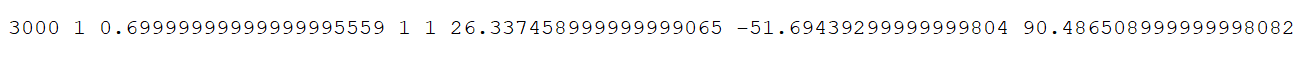
\includegraphics[width=\linewidth]{Config_Files_original_electric_propulsion_settings.png}}
	\caption{\label{fig:zero_order_coefficient}Original Electric Propulsion Settings.}
\end{figure}

\noindent \knownissuelabel{\textbf{Note: }}{elec_prop_system_name_issue} Currently, the spacecraft options file \ac{EMTG} generated for the LowSIRIS-REx mission names the electric propulsion system in the Stage Unblocked section \texttt{ElectricPropulsionFrom MissionOptions}. However, the name in the Stage Propulsion Library Block is \texttt{ElectricPropulsio nSystemFromMissionOptions}. Remove the word ``System'' from the Stage Propulsion Library Block to avoid \ac{EMTG} throwing an error at runtime because these two names need to be consistent.

\noindent After saving the new spacecraft options file, run \ac{EMTG} (File -\textgreater run, Ctrl+r) and open the solution file and the LowSIRIS-REx solution file in a text editor after the \acs{NLP} solve finishes. Scroll down to the section just above Objective function (line \({}_{\textrm{\symbol{126}}}\)143). Notice that the spacecraft dry mass increased, and the electric propellant used has decreased in the higher-thrust mission compared to the lower-thrust mission! This change will affect other portions of the solution, as well.


%%%%%%%%%%%%%%%%%%%%%
\section{LowSIRIS-REx Low C3}
\label{sec:lowsiris_rex_low_c3}
%%%%%%%%%%%%%%%%%%%%%

Let’s re-run LowSIRIS-REx with a new launch vehicle. When this mission was run to create the earlier tutorial, the launch C3 from Earth was about \(10.4 \mathrm{km^2/s^2}\) for LowSIRIS-REx and \(7.85 \mathrm{km^2/s^2}\) for the chemical-thrust version. (You may have different values.) Let’s modify the launch vehicle configuration. Open the \texttt{default.emtg\_launchvehicleopt} file in your \texttt{Config\_ files/hardware\_models} directory. Copy the \texttt{ExampleRocket} line and paste it just below \texttt{ExampleR ocket} and above \texttt{\#EndHardwareBlock}. Name the launch vehicle \texttt{SmallExampleRocket}. Change the \texttt{C3\_upperbound} variable (variable 6) from 50 to 6.5 (or something lower than the C3 of your converged solutions from the earlier tutorials). Save the file.

\noindent In PyEMTG, switch to the ``Global Options'' tab and rename the mission ``LowSIRIS-REx\_high\_thr ust\_low\_c3''. Switch to the ``Spacecraft Options'' tab and select the ``SmallExampleRocket'' as the ``Launch vehicle'' option (you may need to re-select the ``Launch vehicle library file'' to see the new launch vehicle). 

\noindent Run EMTG (File -\textgreater run, Ctrl+r) and open the solution file in a text editor after the \acs{NLP} solve finishes. Look for the first entry in the Journey 0 trajectory (line \({}_{\textrm{\symbol{126}}}\)18) and scroll over to the C3 column. You should see \(6.5 \mathrm{km^2/s^2}\) as the C3 value (or whatever value you set as the maximum C3 in the launch vehicle configuration file). Scroll down to the spacecraft section. You should see that lowering the C3 also lowered the dry mass and increased the electric propellant required.

\noindent This concludes the tutorial on \ac{EMTG} launch vehicle and spacecraft configuration files. You can now use these files to model real-world thrusters, power systems, and launch vehicles in \ac{EMTG}.


\end{document}